
\chapter{Image analysis} 
 
Creation of sensing machines working in the environment necessitate 
a validation of in the context of physical scenarios. Some of these 
scenario are flooding, insect clouds, pollutions, fires.

The focus of this chapter are tools and methods allowing to produce inputs
for physical  simulations. These simulations are compute intensive. It is expected
that they could be achieved using discrete computation models such as
cellular automata. It is expected that they will cooperate with network simulations
in various ways: production of stimuli on sensors, or dangers for the sensor network
itself.

The interest of image anlysis is to produce regions that share similar characteristics.
Analysis follows a conventional flow, starting from a picture coming from sources such as
photographies, maps, radar images, to obtain regions of interests, on which physical simultaion will
take place.


\begin{figure}[hbtp]
\begin{center} 
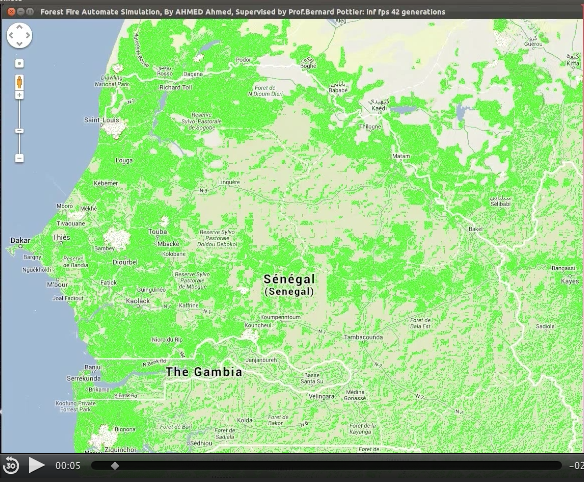
\includegraphics[width=10cm]{AhmedFire.png}
\caption{Fire simulation (or locust expansion) using Cellular Automata implementing  states such as:
vegetation, burning, ashes.}
\label{fig:AhmedFire}
\end{center}
\end{figure}

An example of processing on such regions are cellular automata
reproducing fire expansions of phenomenons consuming characteristics such as the existence od enough vegetation;;
Figure \ref{fig:AhmedFire} is extracted from a
movie demonstration where "fires" are started randomly to "eat" such vegetation report \cite{AhmedFire}. The
work was achieved on an Nvidia GPU.


\section{General flow}

Thus,   modeling  physical regions automatically, or semi-automatically, following physical process 
characteristics, is certainly critical to lead both physical and control network  simulations jointly,
and synchronously. One can think of this as a sampling technique of the physical process sharing
a clock with the sensing network. Cellular automata are one way to implement the real world simulation,
starting from initial states and regions.


A general flow to obtain such regions, is :
\begin{enumerate}
\item  preprocessing  images 
\item segmenting images into blocks
\item recognition of similar cells and grouping into regions
\item processing regions an obtaining skeleton images
\end{enumerate}

Following this flow, higher level objects can be obtained, still with geographical definition in the case of
maps, or satellite imagery.

\section {Preprocessing for image preparation }

In the cas of maps, geographic information is yet presented in a comprehensive way. However analyzing maps is still useful
to obtain information without the direct contact of an initial information system.
More difficult is the case of satellite or plane images, because the contract between objects necessitate
pre processing. Figure \ref{fig:sideBySide} shows an example of procesing achieved using common tools
for management of photographies. The initial view is a satellite image (left), while the right part displays an improved
view, with better contrasts.

\begin{figure}[hbtp]
\begin{center} 
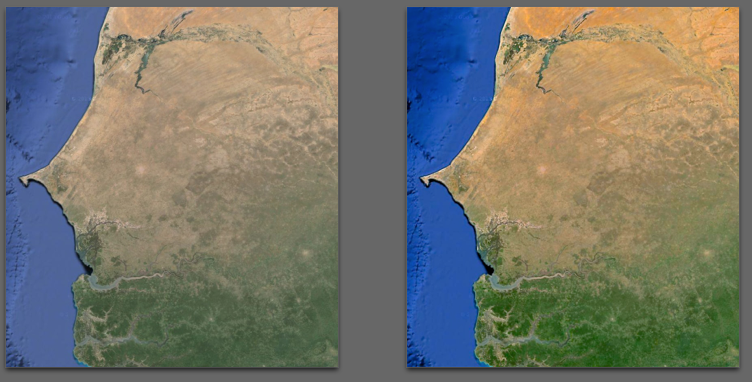
\includegraphics[width=10cm]{SenegalSideBySide.png}
\caption{Modifying original image for better contrasts or coulour selections. Image is a satellite view from Google Maps.}
\label{fig:sideBySide}
\end{center}
\end{figure}

These representations are coming from a very common image processing software 
allowing to change contrasts and colour mapping to fit tne necessity of the recognition.
Image processing paramers show the Red Green Blue statistic values in the original
and the modified image, with a better use of the value range in the second case
(Figure \ref{fig:colours1+2}).



\begin{figure}[hbtp]
\begin{center}
\leavevmode 
\begin{minipage}{6cm}
\begin{center} 
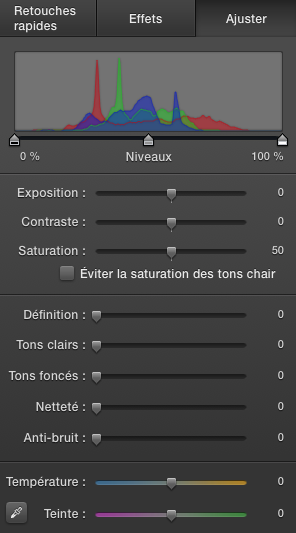
\includegraphics[width=6cm]{senegalColours.png} 
\end{center}
\end{minipage}~~~~~~~~~\begin{minipage}{6cm}
\begin{center} 
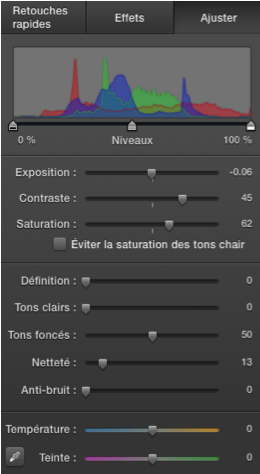
\includegraphics[width=6cm]{senegalColours2.png} 
\end{center}
\end{minipage}
\caption{RGB colour statistics for the left original picture, and its adaptation (right). The software
is Apple iPhoto, standard to any MacOs computer. Similar functions could be obtained from Linux GIMP,
and probably reimplemented from a Palette tool in NetGen.}
\label{fig:colours1+2}
\end{center}
\end{figure}
  
\section { Segmenting the image}

To obtain regions, it is necessary to group zones of the image based on similarities of different kind.
The first operation is a fragmentation into blocks of different size and geometry. Of course,
squares, or rectangles are the simplest way to proceed, but other fragmentation techniques could also
be suitable and ease further stages in simulation. Cellular automata propose as example  an hexagonal
shape where each cell has 6 direct neighbours.

{\sc PickCell} has been implemented (and is till implemented to ease this fragmentation, in relation with 
further networks definition.

This tool reuse the {\sl Picking} framework presented Figure  \ref{fig:PickPoint1}. Beside the capability
to load images, and specify sensor positions, there is the ability to install a rectangular grid over the
image.


\begin{figure}[hbtp]
\begin{center} 
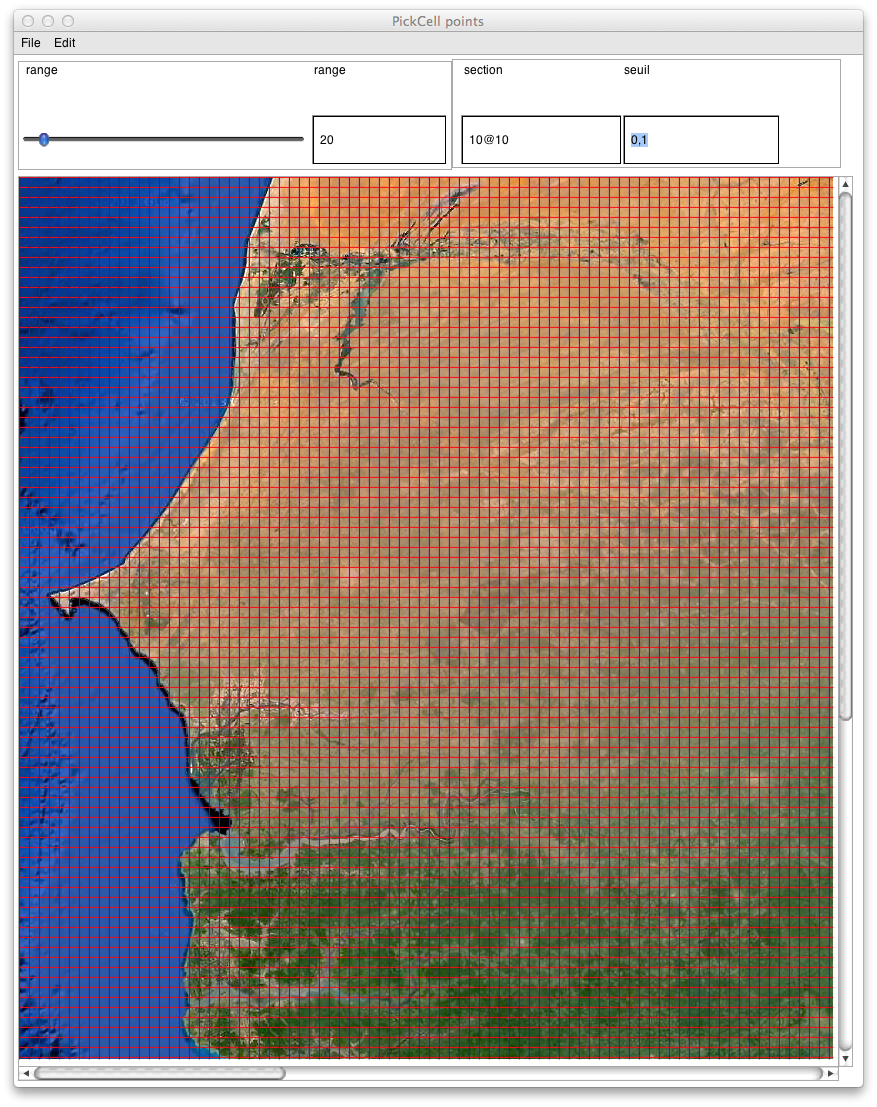
\includegraphics[width=10cm]{SenegalGrid10x10.png}
\caption{Using a 10@10 grid, the image is split into $10\times10$ pixels. 
Following the application, it is possible to specify $x  \times   y$ grids with $x  \neq  y$.}
\label{fig:SenegalGrid10x10}
\end{center}
\end{figure}

Having split the image into cells, it is now possible to classify thems around common properties.

\begin{figure}[hbtp]
\begin{center} 
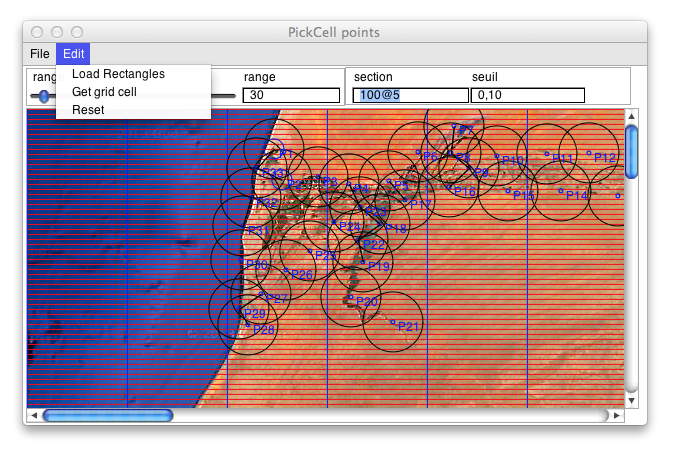
\includegraphics[width=10cm]{SenegalGetGridCell.png}
\caption{Rectangular grid, and sensor geometry specification. The Edit Menu {\sl Get Grid Cell} allows to go a step forward in the flow
to group cell togethers and form {\sl regions} of interest. Section \ref{sec:classification}}
\label{fig:SenegalGetGridCell}
\end{center}
\end{figure}

\section { Grouping block into classes}
\label{sec:classification} 

From the menu shown Figure  \ref{fig:SenegalGetGridCell}, we obtain a new tool for region
specification and manipulation. As for the grid in segmentation, a new parameter allows to divide
the cell space according to pixel distributions.The choice of group distribution  can be more or less sophisticated.
To start by the begining, the following algorithm is applied to the whole cell grid, to obtain a set of $min, max, mean$ parameters
on each colour :

\begin{lstlisting}  
STEP 1
	for each cell in the grid
		for each pixel in the cell 
			 for each colour component in { R, G, B}
				 update (min(colour))
				 update (max(colour))
				 update (sum(colour))
		 for each colour component in { R, G, B}
			 update (mean(colour))
\end{lstlisting}

Following this step, we have $3 \times 3$ parameters set in each cell, thus allowing to compute
global image characteristics that will reflect the efficiency of the preprocessing:

\begin{lstlisting}  
STEP 2
	for each cell in the grid
		for each colour component in { R, G, B}
			update(minGlobal)
			update(maxGlobal)
			update(minMeanGlobal)
			update(maxMeanGlobal)
\end{lstlisting}

